\section{Der Gleichstellungsrat Physik}
Der Gleichstellungsrat Physik hei\ss t alle Erstsemester herzlich willkommen an der Goethe-Universität Frankfurt.\\
Der Gleichstellungsrat Physik setzt sich im Moment aus sieben gewählten
Frauen zusammen. Sie vertreten die Statusgruppen der Studentinnen, der
wissenschaftlichen und technisch-administrativen Mitarbeiterinnen und
der Professorinnen. Diese werden, je nach Statusgruppe, alle ein bis zwei Jahre von der Frauenvollversammlung der Physik gewählt. Die nächste Wahl findet übrigens im kommenden Frühjahr statt.\\
Wir setzen uns für die Themen Chancengleichheit und Familienförderung ein und unterstützen Studierende und Mitarbeiter/innen in allen Lebenslagen. Au\ss erdem engagieren wir uns für viele spannende Projekte wie den Girls' Day oder die Lunch Talks der technisch-administrativen Mitarbeiter/innen. Wir unterstützen die Teilnahme an verschiedenen Tagungen, zum Beispiel der Deutschen Physikerinnentagung oder der Zusammenkunft aller Physik-Fachschaften (ZaPF). Unsere ausleihbare Spielkiste hat schon manchem Elternteil, das spontan sein Kind mit zur Arbeit bringen musste, den Tag gerettet.\\
Speziell für euch Erstsemester bieten wir das Mentoringprogramm Ersti-Hilfe an. Jeder Mentee wird dabei ein Semester lang von einer Kommilitonin oder einem Kommilitonen aus den höheren Semestern durch das Studium begleitet. So können zum Beispiel Fragen zum Zeitmanagement geklärt werden, es gibt viele Tipps und Tricks für das Studium und ihr gewinnt im besten Fall einen Ansprechpartner für eure gesamte Studienzeit. Anmeldung per formloser E-Mail an \url{ersti-hilfe@physik.uni-frankfurt.de}.\\
Weitere Informationen, unsere Kontaktdaten und wie man bei uns mitmachen kann, findet ihr auf unserer Webpage \url{http://goethe.link/gsr-physik}.\\
Wir wünschen euch viel Erfolg im Studium und hoffen, euch bald kennenzulernen!\\
\von{Euer Gleichstellungsrat Physik}
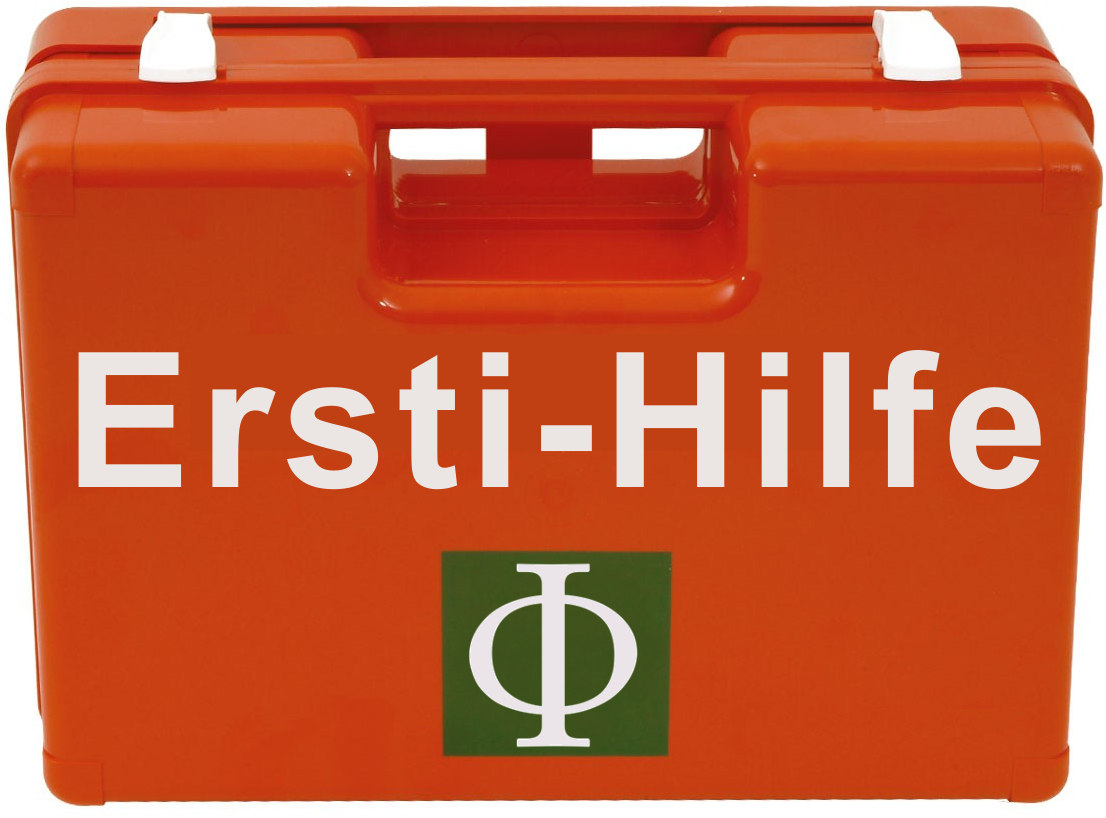
\includegraphics[width=0.5\textwidth]{\imgdir/ersti-hilfe.png}